 
% Copyright 2004 by Till Tantau <tantau@users.sourceforge.net>.
%
% In principle, this file can be redistributed and/or modified under
% the terms of the GNU Public License, version 2.
%
% However, this file is supposed to be a template to be modified
% for your own needs. For this reason, if you use this file as a
% template and not specifically distribute it as part of a another
% package/program, I grant the extra permission to freely copy and
% modify this file as you see fit and even to delete this copyright
% notice. 
\AtBeginDocument{\renewcommand{\bibname}{References}}

\documentclass{beamer}
%\usepackage[table]{xcolor}
\usepackage[absolute,overlay,showboxes]{textpos}
\usepackage{caption}
\usepackage{xcolor,colortbl}
\usepackage{amsmath}
%\usepackage{lipsum}
%\AtBeginDocument{\renewcommand{\bibname}{References}}

% There are many different themes available for Beamer. A comprehensive
% list with examples is given here:
% http://deic.uab.es/~iblanes/beamer_gallery/index_by_theme.html
% You can uncomment the themes below if you would like to use a different
% one:
%\usetheme{AnnArbor}
%\usetheme{Antibes}
%\usetheme{Bergen}
%\usetheme{Berkeley}
%\usetheme{Berlin}
%\usetheme{Boadilla}
%\usetheme{boxes}
%\usetheme{CambridgeUS}
%\usetheme{Copenhagen}
%\usetheme{Darmstadt}
\usetheme{default}
%\usetheme{Frankfurt}
%\usetheme{Goettingen}
%\usetheme{Hannover}
%\usetheme{Ilmenau}
%\usetheme{JuanLesPins}
%\usetheme{Luebeck}
%\usetheme{Madrid}
%\usetheme{Malmoe}
%\usetheme{Marburg}
%\usetheme{Montpellier}
%\usetheme{PaloAlto}
%\usetheme{Pittsburgh}
%\usetheme{Rochester}
%\usetheme{Singapore}
%\usetheme{Szeged}
%\usetheme{Warsaw}

\title{Power Allocation and Relay Selection in
Amplify-and-Forward Relaying
}

% A subtitle is optional and this may be deleted
%\subtitle{Dual Degree Phase 1 Presentation}

\author{Prudhvi Porandla \\ \quad (110070039)\\
\vspace{2mm}
Guide: Prof. Prasanna Chaporkar} 
% - Give the names in the same order as the appear in the paper.
% - Use the \inst{?} command only if the authors have different
%   affiliation.

% - Use the \inst command only if there are several affiliations.
% - Keep it simple, no one is interested in your street address.

%\date{2nd May 2016}
% - Either use conference name or its abbreviation.
% - Not really informative to the audience, more for people (including
%   yourself) who are reading the slides online

%%%%%\subject{Theoretical Computer Science}
% This is only inserted into the PDF information catalog. Can be left
% out. 

% If you have a file called "university-logo-filename.xxx", where xxx
% is a graphic format that can be processed by latex or pdflatex,
% resp., then you can add a logo as follows:

% \pgfdeclareimage[height=0.5cm]{university-logo}{university-logo-filename}
% \logo{\pgfuseimage{university-logo}}

% Delete this, if you do not want the table of contents to pop up at
% the beginning of each subsection:


% Let's get started
\begin{document}

\begin{frame}
  \titlepage
\end{frame}

\begin{frame}{Overview}
  \begin{itemize}
  \item Introduction
  \vspace{3mm}
  \item Relaying Schemes 
  \vspace{3mm}
  \item Power Allocation
  \vspace{3mm}
  \item Relay Selection 
  \vspace{3mm}
  \item Interdependence of above
  \vspace{3mm}
  \item Future Work
  \end{itemize}
  % You might wish to add the option [pausesections]
\end{frame}

% Section and subsections will appear in the presentation overview
% and table of contents.



\begin{frame}{Introduction}
  \begin{itemize}
  \item D2D and Relaying cooperative communications will play important roles in future generation wireless networks.
  \vspace{0.5cm}
  \item Current standard allows deployment of fixed relays to help cell-edge users. 
  \vspace{0.5cm}
  \item Advanced cellular relaying modes like mobile relaying, multi-hop relaying, 
	  and user-assisted relaying are expected in 5G systems.
		  \vspace{0.5cm}
  \item We will discuss the signalling mechanisms in PDF and AF relaying schemes 
\item  We will discuss power allocation and relay selection in AF scheme
  \end{itemize}
  % You might wish to add the option [pausesections]
\end{frame}
%%%%\section{Second Main Section}

\begin{frame}{Partial Decode-and-Forward Relaying} {Two Phases}
Total transmission period is divided into phases: 1. Broadcast phase and 2. Multicast phase as shown in the figure below.
\begin{figure}
\centering
\includegraphics[width=\textwidth]{figures/pdfRelaying.png}
  \caption{Two phases in PDF relaying.}
\end{figure}
\end{frame}

\begin{frame}{Partial Decode-and-Forward Relaying} {Transmit Signals}
Source uses superposition coding and splits its information into a
	common part($U_s^b$) and a private part($V_s^m$) \\ 
	\vspace{1cm}
The signals transmitted by source and relay are as follows:
\begin{align*}
\text{Phase 1:}\quad x^b_s &=  U_s^b, \\
\text{Phase 2:}\quad x_r^m &= U_s^{m}, \\ 
 x^m_s &= U_s^{m} + V_s^{m} 
\end{align*}
\vspace{-0.5cm}
\end{frame}

\begin{frame}{Partial Decode-and-Forward Relaying} {Received Signals}
\vspace{-1cm}
Signals received at relay, BS during broadcast(b) and multicast(m) phases:
\begin{equation*}
Y_r^b = h_{sr}x^b_s + Z_r^b , \quad Y_d^b = h_{sd}x^b_s + Z_d^b
\end{equation*}
$Z_r^b$ and $Z_d^b$ are \textit{i.i.d} $\mathcal{CN}(0,\sigma^2)$ that represent noises at $\mathcal{R}$ and $\mathcal{D}$. \\
\pause
\begin{equation*}
Y_d^m = h_{sd}x^m_s + h_{rd}x_r^m + Z_d^m
\end{equation*}
The above expression is true only if $\mathcal{D}$ has knowledge about the phase offset between $\mathcal{S}$ and $\mathcal{R}$. 
\end{frame}

\begin{frame}{Amplify-and-Forward } {Two Slots}
\begin{figure}
\centering
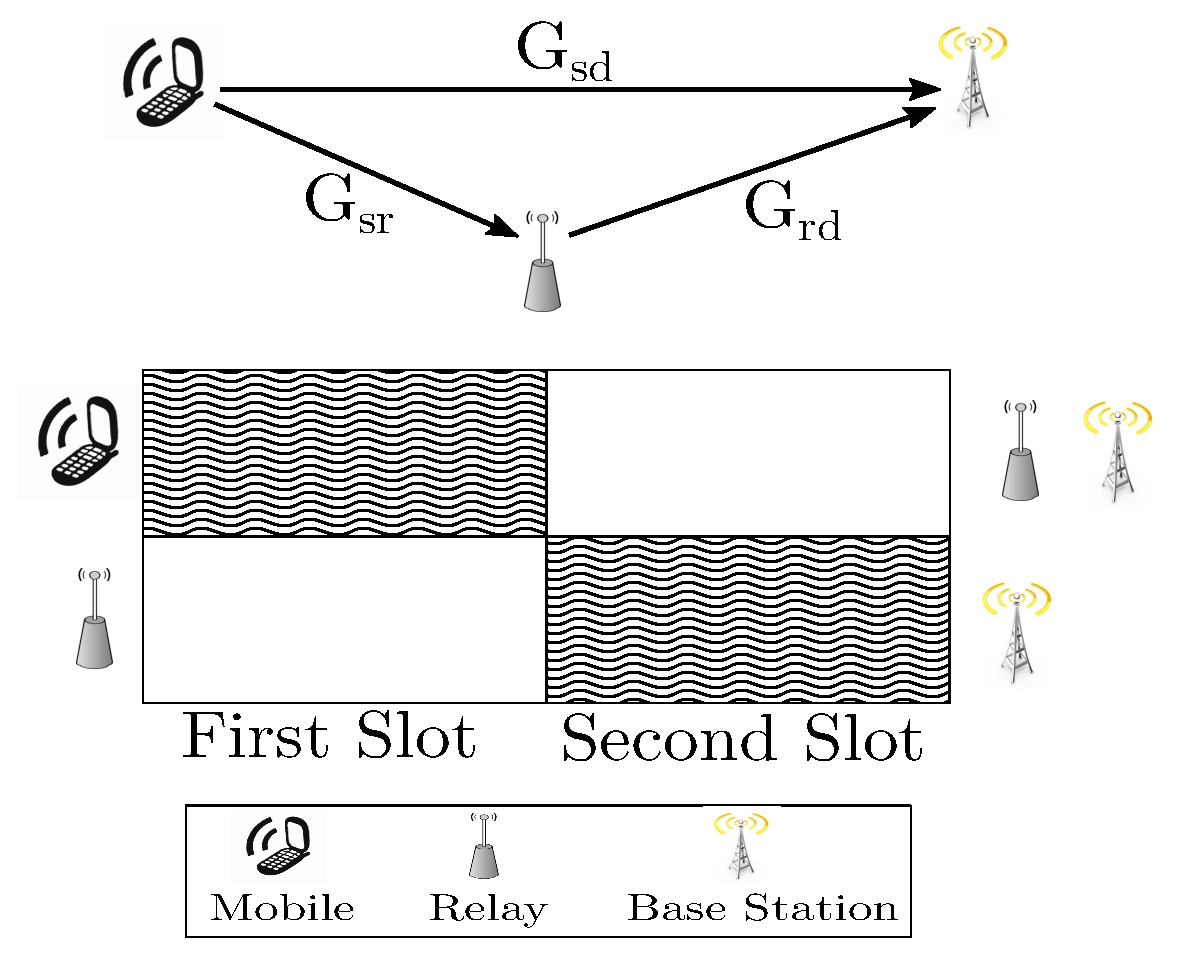
\includegraphics[width=2.5in]{../img/sysmodel.eps}
  \caption{Two phases in AF relaying.}
\end{figure}
\end{frame}

\begin{frame}{Amplify-and-Forward} {Received Signals}
\vspace{-1cm}
Signals received at relay, BS during the two slots: \\
	\textit{First Slot:}
	\begin{align*} 
			Y_{sd} &= \sqrt{P_s G_{sd}} X_s + n_{sd} \\
			Y_{sr} &= \sqrt{P_s G_{sr}} X_s + n_{sr} \\
	\end{align*}
	\textit{Second Slot:}
	\begin{equation*}\label{yrd}
			Y_{rd} = \sqrt{P_r G_{rd}} X_{rd} + n_{rd} 
	\end{equation*}
	Where $X_{rd} = \frac{Y_{sr}}{|Y_{sr}|}$ 
\end{frame}

\begin{frame}{Amplify-and-Forward} {Capacity}
\vspace{-1cm}
The rate/capacity of AF relaying scheme is given by
	\begin{align*}
			R = \frac{1}{2} w \log_2(1+\Gamma_{sd}+\Gamma_{rd}) 
				\\ \text{where $\Gamma$
				represents SNR}
	\end{align*}
	Substituting $\Gamma_{sd}$ and $\Gamma_{rd}$, we get 
	\begin{align*}
			R &= \frac{1}{2} w \log_2\bigg(1+\frac{P_s G_{sd}}{\sigma^2} +
				\frac{P_s G_{sr} P_r G_{rd}}{\sigma^2(\sigma^2 + P_sG_{sr} + P_rG_{rd})}\bigg)
	\end{align*}
\end{frame}

\begin{frame}{Power Allocation}{Single relay case}
	\vspace{1cm}
	\begin{itemize}  
  \item
	  Find the source power that maximises rate under given power constraints
  \vspace{1cm}
  \pause
  \item Prove that rate is concave function of source power
  \pause
  \vspace{1cm}
  \item Use Lagrange multiplier method to find optimal power 	

	\end{itemize}
\end{frame}

\begin{frame}{Power Allocation}{Multiple relays}
	\vspace{-1cm}
	Depends on the relay
\end{frame}

\begin{frame}{Relay Selection}
	\vspace{-1cm}
Many relay selection schemes. One of them: \\ 
	\vspace{1cm}
	Select relay $k$
where 
	\begin{equation*}
		k = \arg \max\min\limits_{i} \{ G_{sr_i},G_{r_id} \} 
	\end{equation*}
	\pause
	A smoother version of the above would be
	\begin{equation*}
		k = \arg \max\limits_{i} \frac{ G_{sr_i}G_{r_id} }{ G_{sr_i}+G_{r_id} } 
	\end{equation*}
	
\end{frame}

\begin{frame}{Relay Selection}{Optimal Scheme}
	\vspace{-1cm}
	An optimal scheme should use SNR as the deciding parameter \\
	In our case \\
Select relay $k$
where 
	\begin{equation*}
		k = \arg \max\limits_{i} \Gamma_{r_id}
	\end{equation*}
	where $\Gamma_{rd} = \frac {P_s G_{sr} P_r G_{rd}}{\sigma^2(\sigma^2 + P_sG_{sr} + P_rG_{rd})}$	
\end{frame}


\begin{frame}{Interdependence}
	\vspace{-1cm}
	Power allocation and relay selection mutually dependent
	\vspace{1cm}
	Can different relays be optimal at different
	source powers?
\end{frame}

\begin{frame}{}
consider two
relays $R_1$ and $R_2$ and assume both use same constant relay power $P_r$.
	$\Gamma_{rd}$ can be rewritten as
	\begin{equation*}
			\Gamma(P_s) = \frac{P_s ab}{1+P_s a + b} 
	\end{equation*}
	where $a = \frac{G_{sr}}{\sigma^2}$ and $b = \frac{P_{r} G_{r d}}{\sigma^2}$
\\
	We want to know if at some power $P_1$, $R_1$ is a better
	relay than $R_2$ i.e., \\ $\Gamma_1(P_1) > \Gamma_2(P_1)$ \\ then can $R_2$ be 
	a better relay than $R_1$ for some other power $P_2$? \\
	$\Gamma_1(P_2) < \Gamma_2(P_2)$
\end{frame}
\begin{frame}
let us find the power at which both relays are equally good.
	\begin{align*}
			\Gamma_1(P_0) = \Gamma_2(P_0)
	\end{align*}
	Solving the above equation, we get
	\begin{equation*}
			P_0 = (1+b_1)(1+b_2) \frac{\frac{a_1b_1}{1+b_1} - 
				\frac{a_2b_2}{1+b_2}}{a_1a_2(b_2-b_1)}
	\end{equation*}
\end{frame}
\begin{frame}
	For $P_0$ to be positive, both numerator and denominator should 
	have same sign i.e., if 
	$\frac{a_1b_1}{1+b_1} >	\frac{a_2b_2}{1+b_2}$ then $b_2 > b_1$.
	To explain this intuitively, let us assume $b_1,b_2$ to be 
	much larger than 1 which reduces the first inequality to
	$a_1 > a_2$. What this means is, source to relay channel is 
	better for $R_1$ but relay to destination channel is stronger
	for $R_2$. Hence at low source powers $R_1$ gives
	better SNR but for  source power greater than  $P_0$, $R_2$ 
	is a better relay than $R_1$. Same argument can be made 
	for the case where inequalities are in the opposite
	direction. 
	\\
\end{frame}
\begin{frame}
	For $P_0 < 0$, one of the relays is the desired one irrespective of source power.
\end{frame}
\begin{frame}
	To summarise, here are the conditions under which one relay is better than the other:
	\begin{itemize}
		\item $\frac{a_1b_1}{1+b_1} >	\frac{a_2b_2}{1+b_2}$ and $b_2 > b_1$ \\
			$R_1$ at source power less than  $P_0$ and $R_2$ at power greater than $P_0$
		\item $\frac{a_1b_1}{1+b_1} < \frac{a_2b_2}{1+b_2}$ and $b_2 < b_1$ \\
			$R_2$ at source power $<P_0$ and $R_1$ at power $>P_0$
		\item $\frac{a_1b_1}{1+b_1} < \frac{a_2b_2}{1+b_2}$ and $b_2 > b_1$ \\
			$R_2$ is a better relay for all source powers
		\item $\frac{a_1b_1}{1+b_1} >	\frac{a_2b_2}{1+b_2}$ and $b_2 < b_1$ \\
			$R_1$ is a better relay for all source powers
	\end{itemize}
\end{frame}

\begin{frame}{}
	\vspace{1cm}
	\begin{itemize}  
		\item
			Assume an initial source power
			\vspace{1cm}
		\item Select the best relay at this power
		\item Solve the optimisation problem
		\item Check if the current relay is still the best
		\item If not use the other relay
	\end{itemize}
\end{frame}


\begin{frame}{Future Work}
	\vspace{1cm}
	\begin{itemize}  
		\item
			Will the above method work?
			\vspace{1cm}
			\pause
		\item Extend it to the case where there are more than two relays
			\pause
		\item Power allocation at relay
	\end{itemize}
\end{frame}


\begin{frame}{}
	\centering
	\textbf{Thank You}
\end{frame}

\end{document}
